\section{Математическое моделирование}


\begin{frame}{Математическая модель пневмопривода}
	\begin{columns}
		\begin{column}{0.6\textwidth}
			\vspace{-0.6cm}
			\begin{block}{\small Ключевые уравнения}
				\scriptsize
				\begin{compactitem}
					\item \textbf{Механика:}
					$
						M\ddot{x} = p_1F_1 - p_2F_2 - p_\text{атм}(F_1 - F_2) - R_\text{тр}(\dot{x}) - R_\text{упор}(x,\dot{x})
					$
					\item \textbf{Трение:}
					$
						R_\text{тр}(\dot{x}) = \sigma_0z + \sigma_1\dot{z} + \sigma_2\dot{x}
					$\\
					где $z = \dot{x} - \frac{\sigma_0|\dot{x}|}{g(\dot{x})}x$ при
					$g(v) = R_\text{к} + (R_\text{с} - R_\text{к})e^{-(|v|/v_s)^\delta}$
					\item \textbf{Упоры:\\}
					$
						R_\text{уп} = \begin{cases}
							k_\text{уп}(x - x_\text{мин}) + b_\text{уп}\dot{x},  & \text{если } x < x_\text{мин}                       \\
							0,                                                   & \text{если } x_\text{мин} \leq x \leq x_\text{макс} \\
							k_\text{уп}(x - x_\text{макс}) + b_\text{уп}\dot{x}, & \text{если } x > x_\text{макс}
						\end{cases}
					$
					\item \textbf{Термодинамика:}
					$
						\begin{aligned}
							\frac{dp_i}{dt} & = \frac{\gamma}{V_i}\left(RT_1(G_{i\text{ вх}} - G_{i\text{ вых}}) - p_i F_i\frac{dx}{dt}\right)     \\
							\frac{dT_i}{dt} & = \frac{\gamma-1}{m_iC_v}\left(RT_i(G_{i\text{ вх}} - G_{i\text{ вых}}) - p_iF_i\frac{dx}{dt}\right)
						\end{aligned}
					$
					\item \textbf{Расход через распределители:\\}
					$
						G_i = \psi(p_1, p_2) \cdot C_d F_{max} \cdot u \frac{p_1}{\sqrt{RT_\text{вх}}}.
					$\\
					Расходная функция $\psi(p_1, p_2)$ определяется через закон Сен-Венана--Ванцеля.
					\item \textbf{Динамика переключении:\\}
					$
						\tau \frac{du}{dt} + u = u_{\text{зад}},
					$

				\end{compactitem}
			\end{block}
		\end{column}

		\begin{column}{0.4\textwidth}
			\scriptsize Система дополняется \textbf{моделью управления} в общем виде:
			\scriptsize $
				u_{\text{зад}} = u(x, \dot{x}, \dots, t)
			$
			\begin{center}
				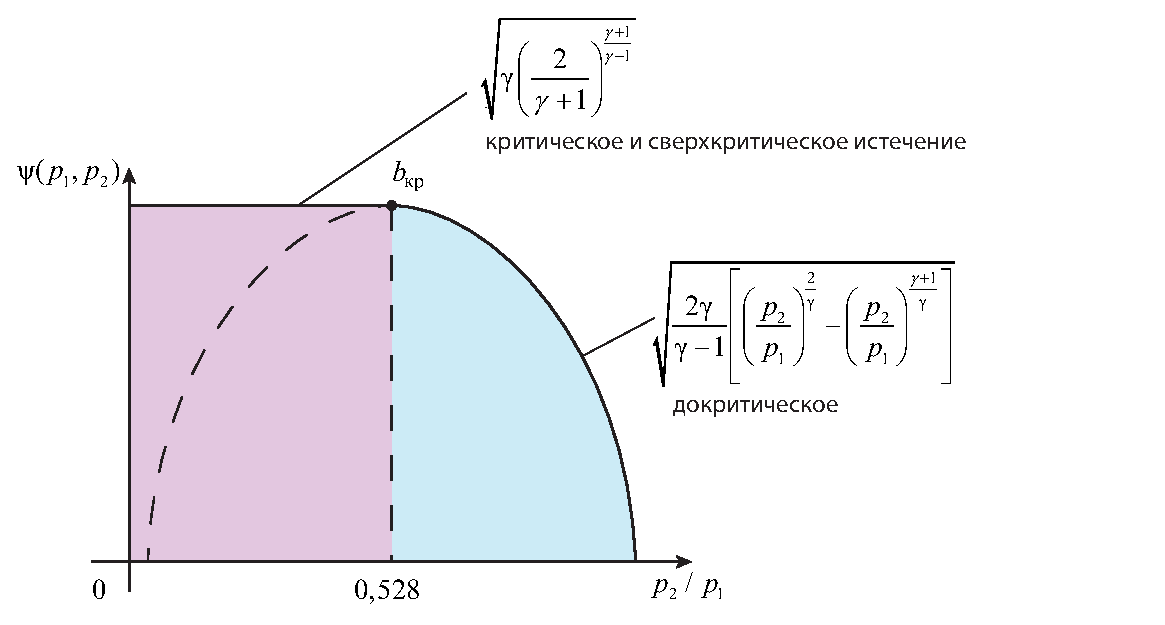
\includegraphics[width=1.3\textwidth]{critical_gas_flow_chart.eps}
				\scriptsize Закон Сен-Венана--Ванцеля
				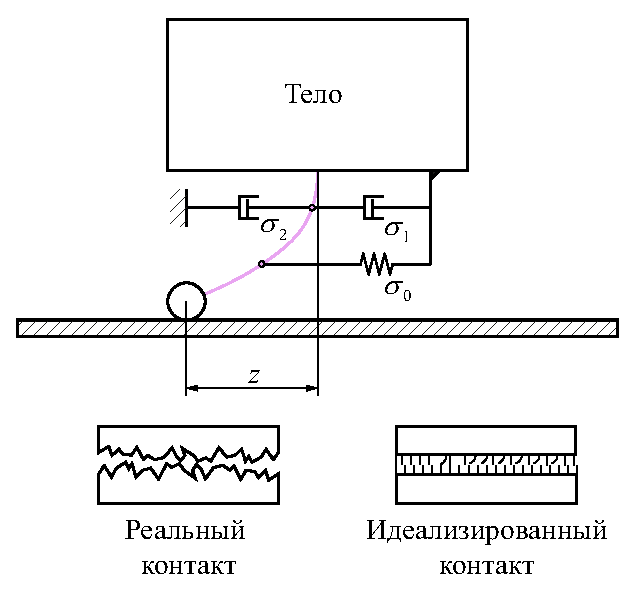
\includegraphics[width=0.8\textwidth]{Трение.eps}
				\scriptsize Модель трения LuGre
			\end{center}
		\end{column}
	\end{columns}
\end{frame}


% \begin{frame}{Полная мат. модель}

% 	\begin{columns}

% 		\begin{column}{0.5\textwidth}
% 			\begin{block}{Система уравнений}
% 				\scriptsize
% 				\begin{equation*}
% 					\begin{cases}
% 						\begin{alignedat}{2}
% 							\dot{x}               & = v                                                                                                                                                                                \\
% 							M\dot{v}              & = \mathbf{F}^T\mathbf{p} - p_\text{атм}(\mathbf{F}^T\mathbf{1}) - R_\text{тр}(v) - R_\text{оп}(x, v)                                                                               \\
% 							\dot{\mathbf{p}}      & = \frac{\gamma}{\mathbf{V}(\mathbf{x})} \odot (R\mathbf{T} \odot \mathbf{G} - \mathbf{p} \odot (\mathbf{F}v))                                                                      \\
% 							\dot{\mathbf{T}}      & = \frac{\gamma-1}{\mathbf{m}C_v} \odot (R\mathbf{T} \odot \mathbf{G} \pm \mathbf{p} \odot (\mathbf{F}v))                                                                           \\
% 							\mathbf{u}_\text{зад} & = \tau \dot{\mathbf{u}} + \mathbf{u}                                                                                                                                               \\
% 							\mathbf{G}            & = \psi(\mathbf{p}_\text{вх}, \mathbf{p}_\text{вых}) \odot \mathbf{C}_d \odot \mathbf{F}_\text{пр} \odot \mathbf{u} \odot \frac{\mathbf{p}_\text{вх}}{\sqrt{R\mathbf{T}_\text{вх}}} \\
% 							R_\text{тр}           & = \sigma_0 z + \sigma_1 \dot{z} + \sigma_2 v                                                                                                                                       \\
% 							\dot{z}               & = v - \frac{\sigma_0 |v|}{g(v)}z                                                                                                                                                   \\
% 							R_\text{оп}           & = k_\text{оп}(x - x_\text{мин})\cdot \frac{1}{1 + e^{-\alpha(x - x_\text{мин})}} +                                                                                                 \\
% 							                      & + k_\text{оп}(x - x_\text{макс})\cdot \frac{1}{1 + e^{-\alpha(x - x_\text{макс})}}
% 						\end{alignedat}
% 					\end{cases}
% 				\end{equation*}
% 			\end{block}
% 		\end{column}

% 		\begin{column}{0.5\textwidth}
% 			\centering
% 			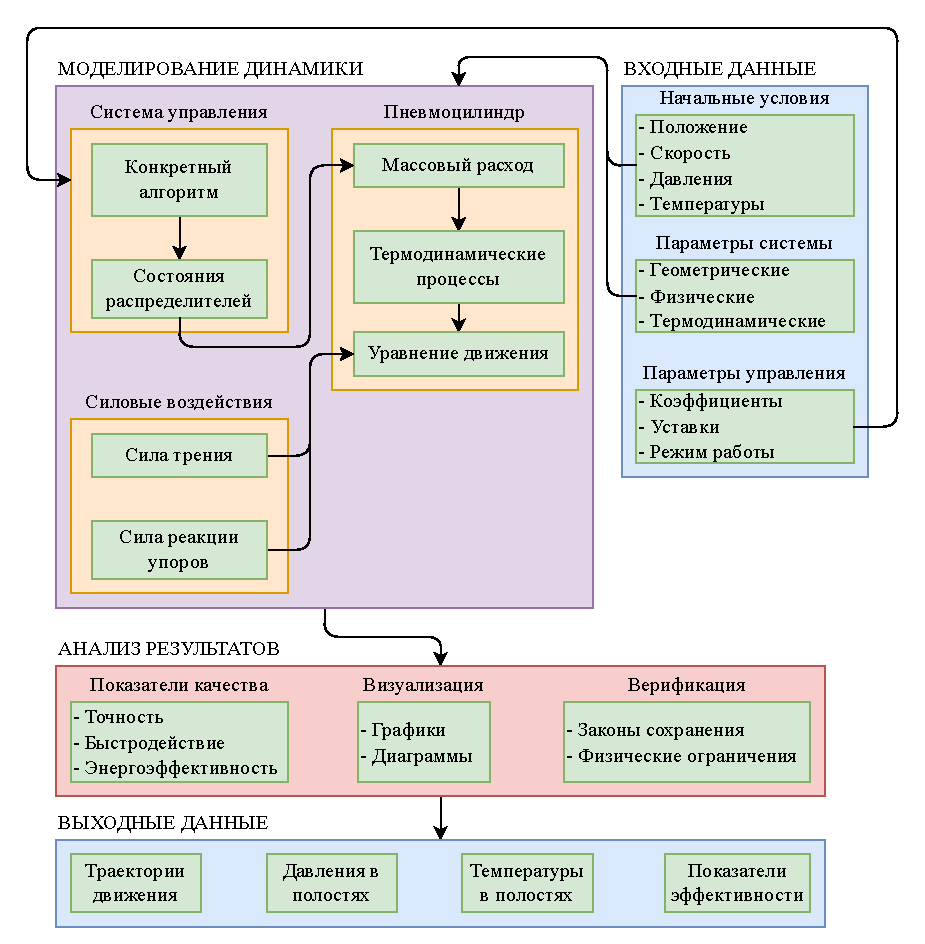
\includegraphics[width=1.1\textwidth]{pneumatic_actuator_functional_block_diagram.pdf}
% 			\text{\small Блок-схема мат. модели}

% 		\end{column}
% 	\end{columns}

% \end{frame}

\begin{frame}
	\frametitle{Исследование режимов работы пневмопривода}
	\begin{columns}
		\begin{column}{0.45\textwidth}
			\begin{block}{Режимы работы}
				\begin{enumerate}
					\item \scriptsize Быстрое выдвижение \hfill [1,0,1,0]
					\item \scriptsize Умеренное выдвижение \hfill [1,0,0,0]
					\item \scriptsize Слабое выдвижение \hfill [0,0,1,0]
					\item \scriptsize Удержание/торможение \hfill [0,0,0,0]
					\item \scriptsize Cлабое втягивание \hfill [0,1,0,0]
					\item \scriptsize Умеренное втягивание \hfill [0,0,0,1]
					\item \scriptsize Быстрое втягивание \hfill [0,1,0,1]
				\end{enumerate}
			\end{block}

			\begin{block}
				\scriptsize Из \textbf{16} возможных комбинаций состояний дискретных распределителей выделены
				и использованы \textbf{7} ключевых режимов движения
			\end{block}

		\end{column}
		\hspace{-0.8cm}
		\begin{column}{0.55\textwidth}
			\centering
			\begin{tabular}{cc}
				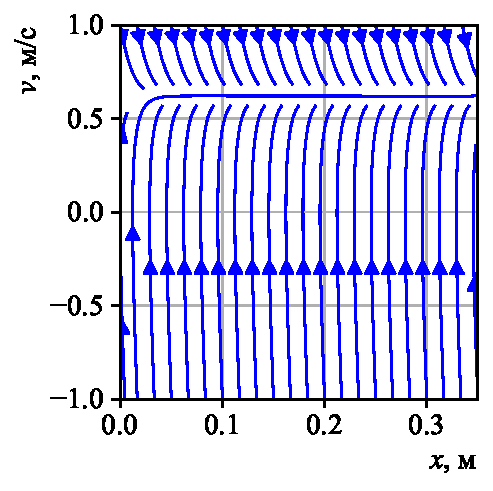
\includegraphics[width=0.45\textwidth]{pp_strong_acceleration_positive.pdf} &
				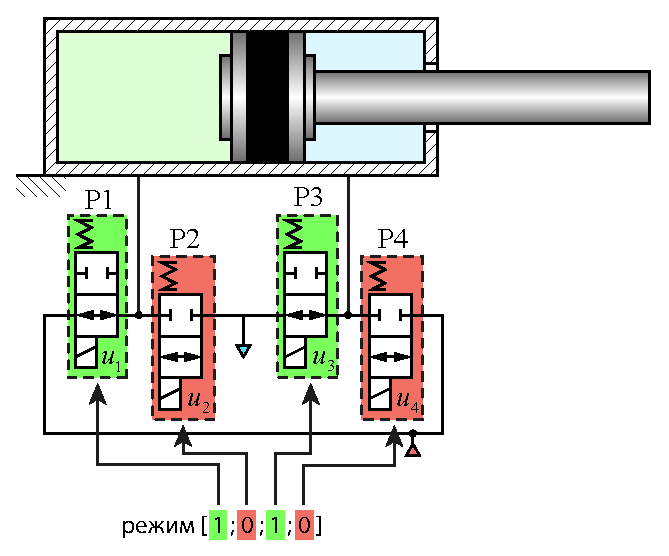
\includegraphics[width=0.5\textwidth]{пример_сильное_ускорение.eps}           \\
				\scriptsize сильное ускорение [1,0,1,0]                                     & \\
				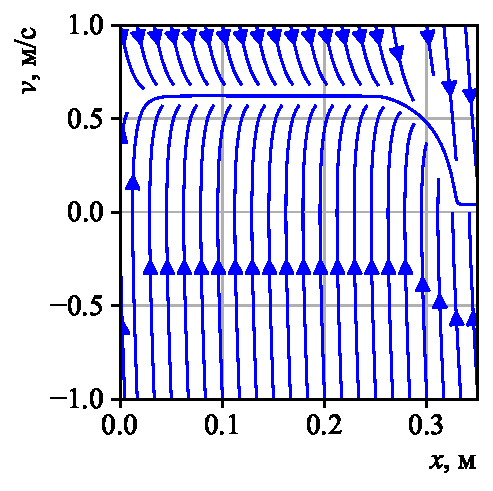
\includegraphics[width=0.45\textwidth]{pp_medium_acceleration_x_01.pdf}     &
				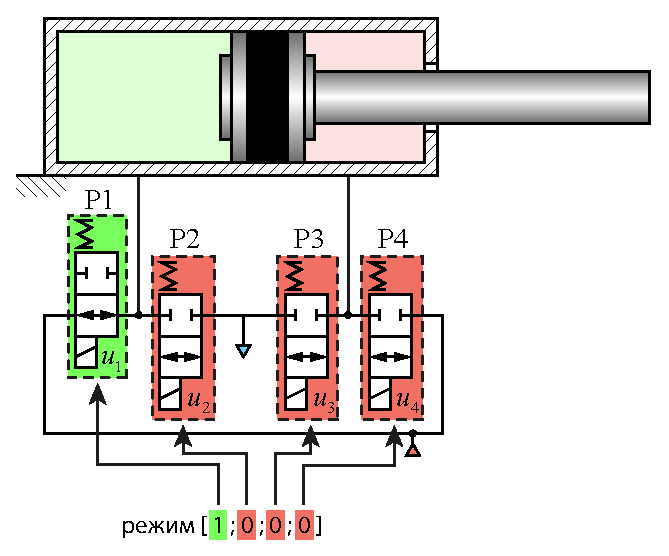
\includegraphics[width=0.5\textwidth]{пример_среднее_ускорение.eps}           \\
				\scriptsize среднее ускорение [1,0,0,0]                                     & \\
			\end{tabular}
			% \includegraphics[width=0.45\textwidth]{}     \\\\
			% \begin{tabular}{cc}
			% 	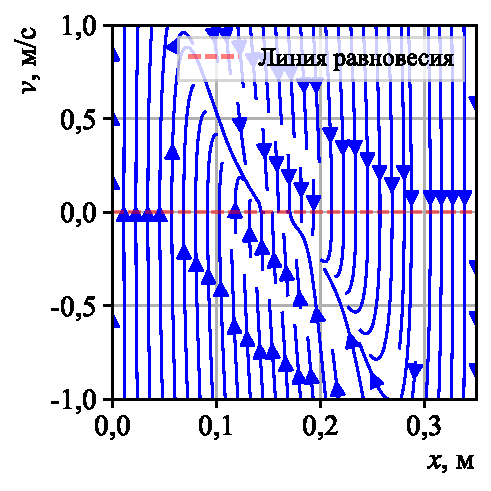
\includegraphics[width=0.45\textwidth]{pp_hold_balanced.pdf}              &
			% 	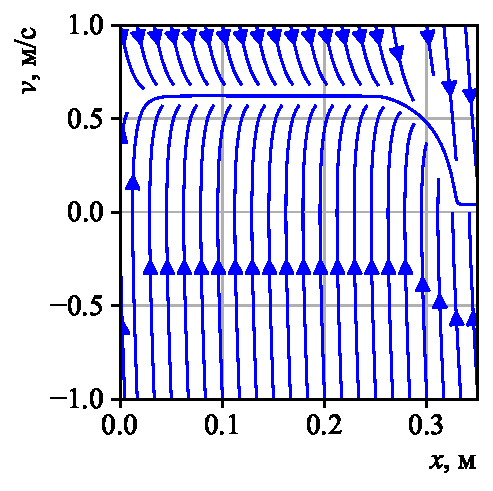
\includegraphics[width=0.45\textwidth]{pp_medium_acceleration_x_01.pdf}                                               \\
			% 	\scriptsize удержание [0,0,0,0]                                           & \scriptsize умеренное ускорение [1,0,0,0] \\
			% 	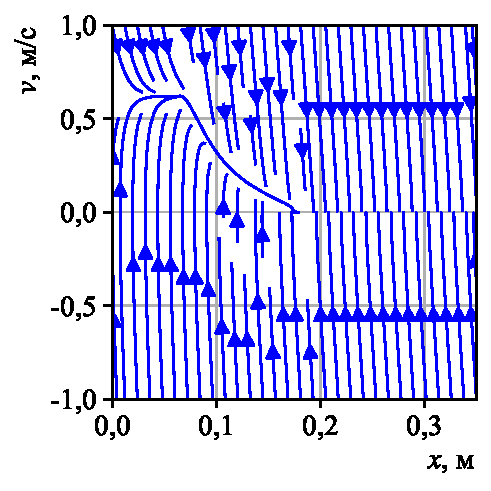
\includegraphics[width=0.45\textwidth]{pp_slow_acceleration_x_01_p_3.pdf} &
			% 	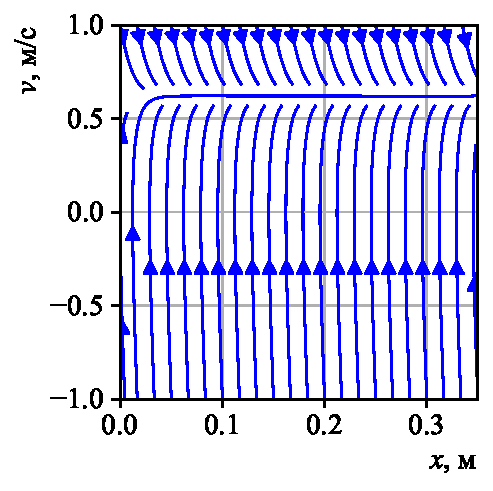
\includegraphics[width=0.45\textwidth]{pp_strong_acceleration_positive.pdf}                                           \\
			% 	\scriptsize слабое ускорение [0,0,0,1]                                    & \scriptsize сильное ускорение [1,0,0,1]   \\
			% \end{tabular}
		\end{column}

	\end{columns}
\end{frame}

\section{Алгоритмы управления}
\begin{frame}
	\frametitle{Модифицированный ПИД-регулятор с ШИМ и адаптивным торможением: структура}

	\begin{columns}[T]
		\begin{column}{0.5\textwidth}
			\vspace{-1em}
			\begin{block}{\scriptsize \textbf{Ключевые модификации}}
				\begin{itemize}
					\item \scriptsize Блок прогнозирования тормозного пути
					\item \scriptsize Адаптивное торможение при подходе к целевой позиции
					\item \scriptsize Анти-насыщение интегральной составляющей
				\end{itemize}
			\end{block}

			\vspace{-0.5em}

			\begin{scriptsize}
				\begin{block}{\scriptsize \textbf{Модель}}
					\textbf{Расчет тормозного пути:}\\
					$	s_{\text{т}}(t) = \frac{v|v|}{2a_{\text{т}}} \cdot \left(1 + 0,2e^{-\frac{|v|}{0.1}}\right)$\\
					\textbf{Модифицированный ПИД:}\\
					$
						u_{\text{пид}} = K_{\text{п}}e + K_{\text{и}}\int\limits_{0}^{t}e(\tau)d\tau\alpha + K_{\text{д}}\beta\frac{de}{dt}
					$\\
					где $\alpha$ -- коэффициент анти-насыщения, $\beta$ -- фильтр производной\\
					\textbf{Интенсивность торможения:}\\
					$
						k_{\text{т}}(t) = \frac{1}{1 + e^{5 \cdot \left(\frac{d_{\text{ц}}}{s_{\text{т}} \cdot k_{\text{п}}} - 0,5\right)}}
					$\\
					\textbf{Результирующее воздействие:}
					$
						u(t) = (1 - k_{\text{т}})u_{\text{пид}} + k_{\text{т}}u_{\text{т}}
					$\\
				\end{block}

			\end{scriptsize}
		\end{column}

		\begin{column}{0.5\textwidth}
			\centering
			\begin{minipage}{\textwidth}
				\centering
				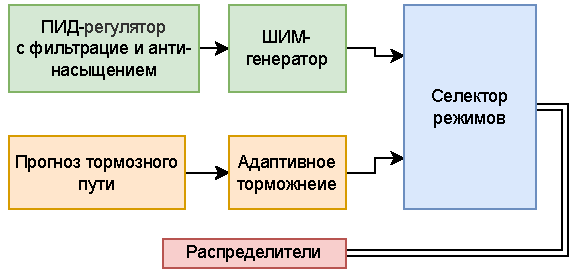
\includegraphics[width=\textwidth]{адаптивное ШИМ управление.pdf}
			\end{minipage}

			\begin{block}{\scriptsize \textbf{Основные преимущества}}
				\scriptsize
				Осуществление торможения при подходе к целевой позиции, улучшение точности позиционирования, увеличение ресурса распределителей
			\end{block}
			% \begin{minipage}{\textwidth}
			% \end{minipage}


		\end{column}

	\end{columns}
\end{frame}

\begin{frame}{Свидетельство ЭВМ}
	\centering
	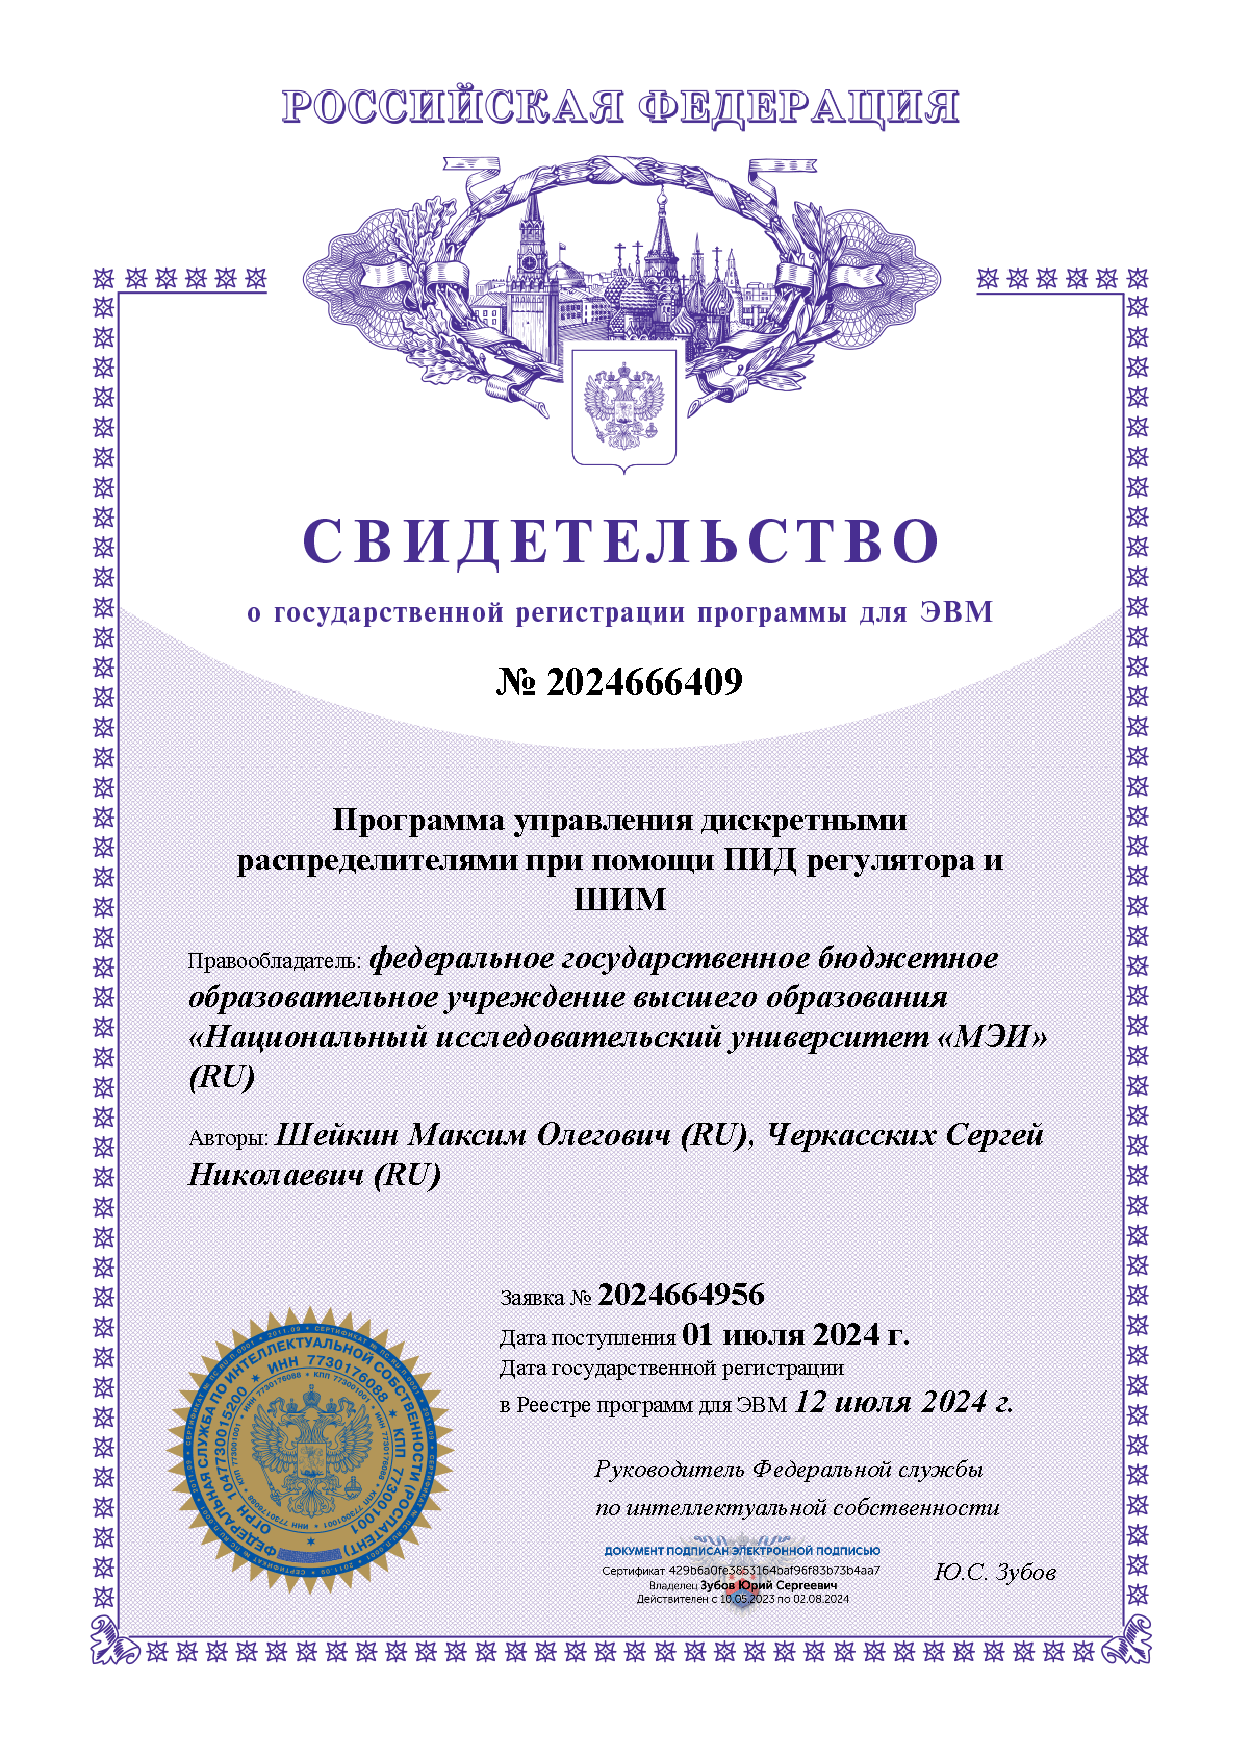
\includegraphics[width=0.5\textwidth]{2024666409.eod.pdf}
\end{frame}


\begin{frame}
	\frametitle{Скользящие режимы}

	\vspace{-0.5cm}

	\begin{columns}[t]
		\scriptsize

		\column{0.5\textwidth}
		\begin{itemize}
			\item Функция переключения: $s = \dot{e} + \lambda e + \gamma\int e dt$
			\item Обеспечение движения по поверхности скольжения $s=0$
			\item Закон управления для 3 режимов:
			      \begin{equation*}
				      \mathbf{u}(s) = \begin{cases}
					      [1,0,0,1], & s > \varepsilon      \\
					      [0,0,0,0], & |s| \leq \varepsilon \\
					      [0,1,1,0], & s < -\varepsilon
				      \end{cases}
			      \end{equation*}
		\end{itemize}

		\vspace{-0.25cm}
		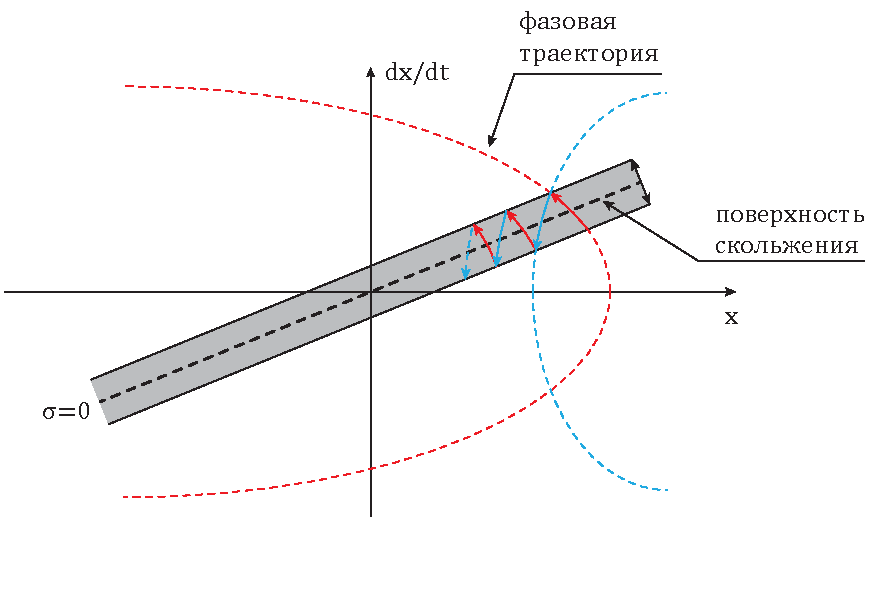
\includegraphics[width=\textwidth]{рис_1_скользящий_режим.pdf}

		\column{0.5\textwidth}
		\begin{block}{\scriptsize\textbf{Типы поверхностей:}}
			\begin{itemize}
				\item Интегральная: $s = \dot{e} + \lambda_1 e + \lambda_2 \int e\, dt$
				\item Терминальная: $s = \dot{e} + \beta |e|^{q/p}\text{sign}(e)$
			\end{itemize}
		\end{block}

		\begin{block}{\scriptsize\textbf{Многорежимное управление:}}
			\begin{itemize}
				\item 3 режима: простота реализации, базовая производительность
				\item 5 режимов: улучшение точности, снижение интенсивности переключений
				\item 7 режимов: наилучшая точность позиционирования (до 0.14 мм)
			\end{itemize}
		\end{block}

		\begin{block}{\scriptsize\textbf{Ключевые особенности:}}
			\begin{itemize}
				\item Высокая робастность к параметрическим возмущениям
				\item Гарантированная устойчивость системы при соблюдении условия скольжения $s\dot{s} < 0$
			\end{itemize}
		\end{block}

	\end{columns}

\end{frame}

\begin{frame}
	\frametitle{Нечеткая логика}

	\scriptsize
	\begin{columns}[T]
		\begin{column}{0.48\textwidth}
			% \textbf{Структура нечеткого регулятора}
			% \begin{center}
			% 	% \includegraphics[height=3.5cm]{images/fuzzy_controller.png}
			% \end{center}

			% \begin{block}{\textbf {\scriptsize Структура нечеткого регулятора}}
			% 	\begin{itemize}
			% 		\item Сигмоидальные и Z функции принадлежности
			% 	\end{itemize}

			% \end{block}

			\begin{block}{\textbf {\scriptsize Параметры нечеткого регулятора}}
				% \begin{itemize}\setlength{\itemsep}{0pt}
				\begin{itemize}
					\item 5 градаций оценок для ошибки
					\item 5 градаций оценок для скорости
					\item 7 команд управления
					\item 25 правил принятия решений
				\end{itemize}
			\end{block}

			\begin{block}{\textbf {\scriptsize Расшифровака оценок}}
				\begin{itemize}
					\item СиП -- сильно положительная
					\item СрП -- средне положительная
					\item СлП -- слабо положительная
					\item Н -- нулевая
					\item СлО -- слабо отрицательная
					\item СрО -- средне отрицательная
					\item CиО -- сильно отрицательная
				\end{itemize}
			\end{block}
		\end{column}

		\begin{column}{0.48\textwidth}
			\textbf{Режимы работы распределителей}

			\centering
			\begin{tabular}{lcccc}
				\midrule
				\textbf{Режим} & \textbf{Р1} & \textbf{Р2} & \textbf{Р3} & \textbf{Р4} \\
				\midrule
				СиП            & 1           & 0           & 1           & 0           \\
				СрП            & 1           & 0           & 0           & 0           \\
				СлП            & 0           & 0           & 1           & 0           \\
				Н              & 0           & 0           & 0           & 0           \\
				СлО            & 0           & 1           & 0           & 0           \\
				СрО            & 0           & 0           & 0           & 1           \\
				СиО            & 0           & 1           & 0           & 1           \\
				\midrule
			\end{tabular}

			\vspace{0.3cm}

			\begin{center}
				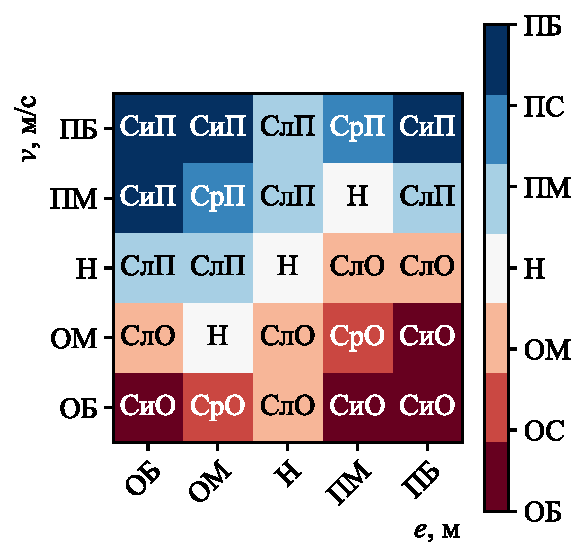
\includegraphics[width=0.75\textwidth]{rule_base_concrete.pdf}
				\\Матрица правил принятия решений
			\end{center}
		\end{column}
	\end{columns}
\end{frame}


\begin{frame}
	\frametitle{Прогнозное управление пневмоприводом: принцип работы}

	\begin{columns}[T]
		\begin{column}{0.48\textwidth}
			\vspace{-1.5em}
			\begin{block}{\small\textbf{Суть метода}}
				\scriptsize
				\begin{itemize}\setlength{\itemsep}{0pt}
					\item Прогнозирование траектории системы
					\item Оптимизация последовательности переключений
					\item Применение только первого шага управления
					\item Повторение процесса на каждом такте
				\end{itemize}
			\end{block}

			% \begin{block}{\small \textbf{Оптимизация}}
			% 	\scriptsize
			% 	\begin{align*}
			% 		J(U) = \underbrace{Q(x - x_{\text{зад}})^2}_{\text{точность}} + \underbrace{R\sum|u_i - u_{i-1}|}_{\text{переключения}}
			% 	\end{align*}
			% \end{block}

			\vspace{-0.6em}
			\begin{exampleblock}{\small \textbf{Ключевые параметры}}
				\scriptsize
				\begin{itemize}\setlength{\itemsep}{0pt}
					\item Горизонт прогноза: $N_p = 8$-$15$
					\item Горизонт управления: $N_u = 2$-$5$
					\item Такт управления: 10-20 мс
				\end{itemize}
			\end{exampleblock}

			\vspace{-0.6em}
			\begin{alertblock}{\small \textbf{Особенности данной реализации}}
				\begin{itemize}
					\item \scriptsize Применяется упрощенная математическая модель для ускорения расчетов
					\item \scriptsize Решается задача оптимизации для нахождения оптимальной последовательности переключений
				\end{itemize}
			\end{alertblock}

		\end{column}

		\begin{column}{0.48\textwidth}
			\begin{center}
				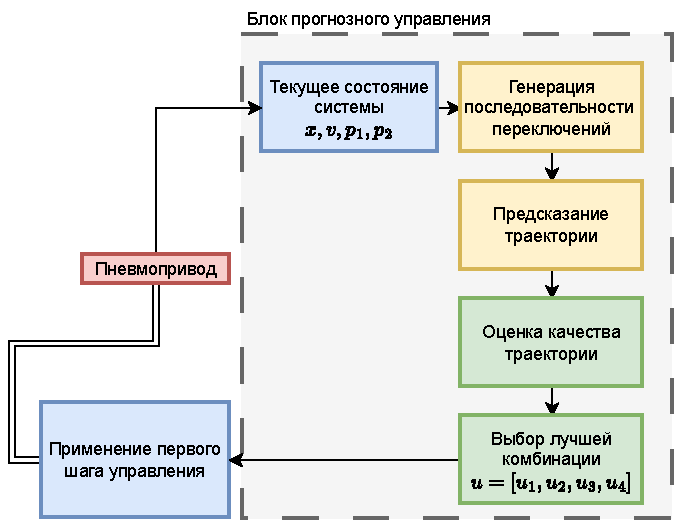
\includegraphics[width=1.15\textwidth]{mpc.pdf}
			\end{center}

		\end{column}
	\end{columns}
\end{frame}

% \begin{frame}
% 	\frametitle{Прогнозное управление пневмоприводом}
% 	\begin{columns}[T]
% 		\begin{column}{0.6\textwidth}
% 			\begin{block}{\small\textbf{Упрощенная модель}}
% 				\scriptsize
% 				$\begin{aligned}
% 						\dot{x}         & = v                                                                                   \\
% 						\dot{v}         & = \frac{1}{M}(p_1A_1 - p_2A_2 - (A_1-A_2)p_a - bv)                                    \\
% 						\dot{p}_1       & = \frac{RT_s}{V_1(x)}(k_g u_1(p_s - p_1) - k_g u_2(p_1 - p_a) - \frac{p_1}{RT_s}F_1v) \\
% 						\dot{p}_2       & = \frac{RT_s}{V_2(x)}(k_g u_3(p_s - p_2) - k_g u_4(p_2 - p_a) + \frac{p_2}{RT_s}F_2v) \\
% 						\tau_v\dot{u}_i & = -u_i + u_{i,cmd}, \quad i = 1,\ldots,4
% 					\end{aligned}$
% 			\end{block}

% 			% \begin{block}{\small \textbf{Ограничения задачи оптимизации}}
% 			% 	\scriptsize
% 			% 	$\begin{aligned}
% 			% 		u_{j,k}                              & \in \{0, 1\}  \\
% 			% 		x_{\text{мин}} \leq x_{k+i}                & \leq x_{\text{макс}} \\
% 			% 		p_{\text{мин}} \leq p_{i,k+j}              & \leq p_{\text{макс}} \\
% 			% 		\sum_{k=1}^{T} |u_{j,k} - u_{j,k-1}| & \leq N_{\text{макс}} \\
% 			% 	\end{aligned}$
% 			% \end{block}

% 		\end{column}
% 		\begin{column}{0.4\textwidth}
% 			\begin{block}{\small\textbf{Оптимизация}}
% 				\scriptsize
% 				\centering
% 				Задача минимизации функционала качества
% 				$\begin{aligned}
% 						J(U) & = \sum_{i=1}^{N_p} Q(x_{k+i} - x_{\text{зад}})^2 +              \\
% 						     & +\sum_{i=0}^{N_u-1}\sum_{j=1}^{4} R_j |u_{j,k+i} - u_{j,k+i-1}|
% 					\end{aligned}$
% 				\begin{itemize}\setlength{\itemsep}{0pt}
% 					\item $N_p$ — горизонт прогноза
% 					\item $N_u$ — горизонт управления
% 					\item $Q$ — вес ошибки позиционирования
% 					\item $R_j$ — вес переключений $j$-го распределителя
% 				\end{itemize}
% 			\end{block}

% 		\end{column}

% 	\end{columns}

% \end{frame}


\section{Экспериментальные исследования}

\begin{frame}{Экспериментальная установка}
	\begin{columns}
		\begin{column}{0.5\textwidth}
			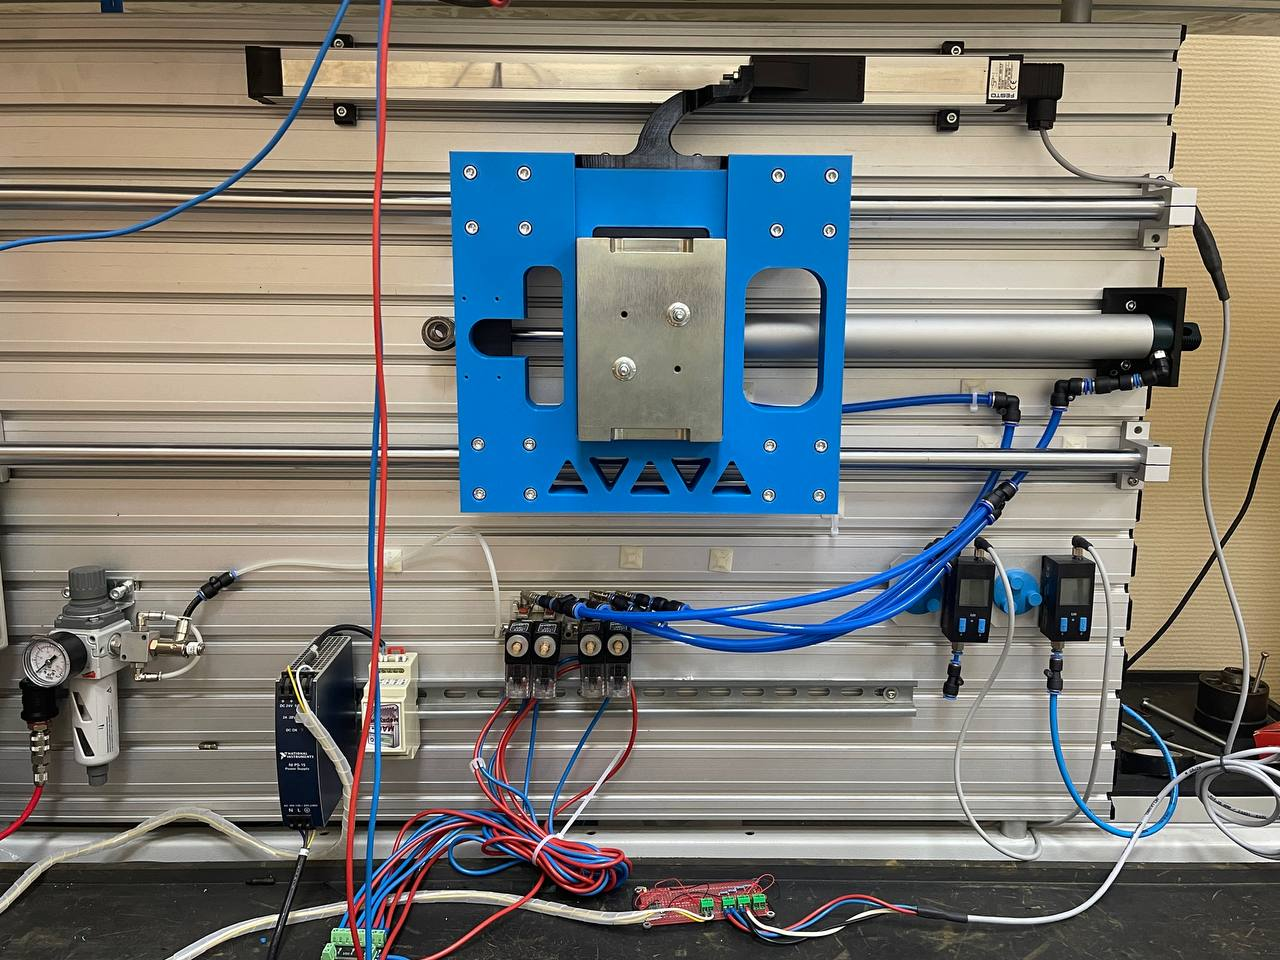
\includegraphics[width=0.95\textwidth]{photo_2025-03-11_14-04-30.jpg}
			\scriptsize{Внешний вид экспериментального стенда}
		\end{column}
		\begin{column}{0.5\textwidth}
			\begin{block}{\scriptsize Параметры}
				\scriptsize
				\begin{itemize}
					\item Пневмоцилиндр: Ø32 мм, ход 350 мм
					\item 4 дискретных распределителя
					\item Датчики положения и давления
					\item Микроконтроллер STM32F767ZI
					\item Веб-интерфейс для управления экспериментом с сервером на RPi 5
				\end{itemize}
			\end{block}
		\end{column}
	\end{columns}

	\vspace{0.2em}

	\begin{minipage}{\textwidth}
		\centering
		\scriptsize
		\begin{tabular}{|l|c|c|}
			\hline
			\textbf{Параметр}            & \textbf{Значение} & \textbf{Единица} \\
			\hline
			Масса платформы              & 1,0               & кг               \\
			Масса груза                  & 5,0               & кг               \\
			Точность измерения положения & 0,0045            & мм               \\
			\hline
		\end{tabular}
	\end{minipage}
\end{frame}

% \begin{frame}{Аппаратная часть и программное обеспечение}
% 	\begin{columns}
% 		\begin{column}{0.48\textwidth}
% 			\centering
% 			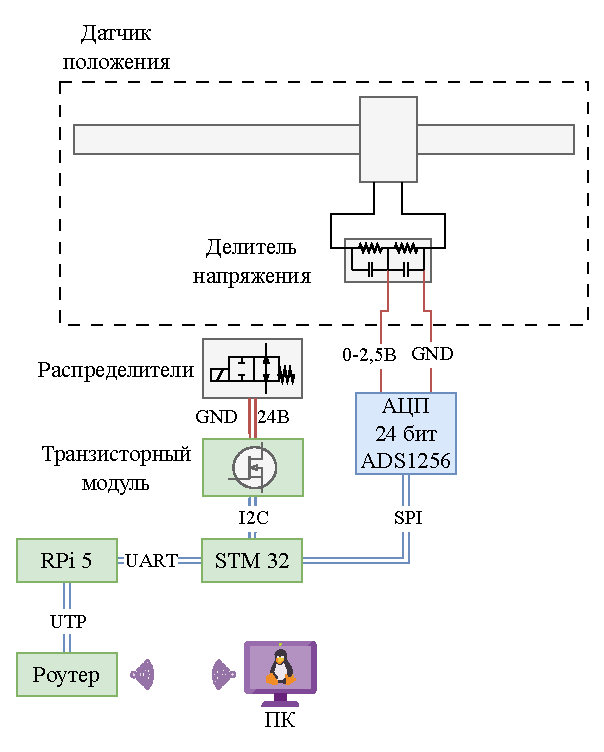
\includegraphics[width=0.75\textwidth]{стурктурная диаграма су.pdf}
% 			\scriptsize{Архитектура системы управления}

% 			\vspace{0.3em}

% 			\scriptsize
% 			\begin{tabular}{|l|l|}
% 				\hline
% 				\textbf{Компонент} & \textbf{Спецификация} \\
% 				\hline
% 				Микроконтроллер    & STM32F767ZI, 216 МГц  \\
% 				АЦП                & 24-бит, 1 кГц         \\
% 				Датчик положения   & Потенциометрический   \\
% 				Датчики давления   & 0-10 бар, класс 0.5   \\
% 				Распределители     & 2/2, 24В DC, 50 Гц    \\
% 				\hline
% 			\end{tabular}
% 		\end{column}
% 		\begin{column}{0.52\textwidth}
% 			\centering
% 			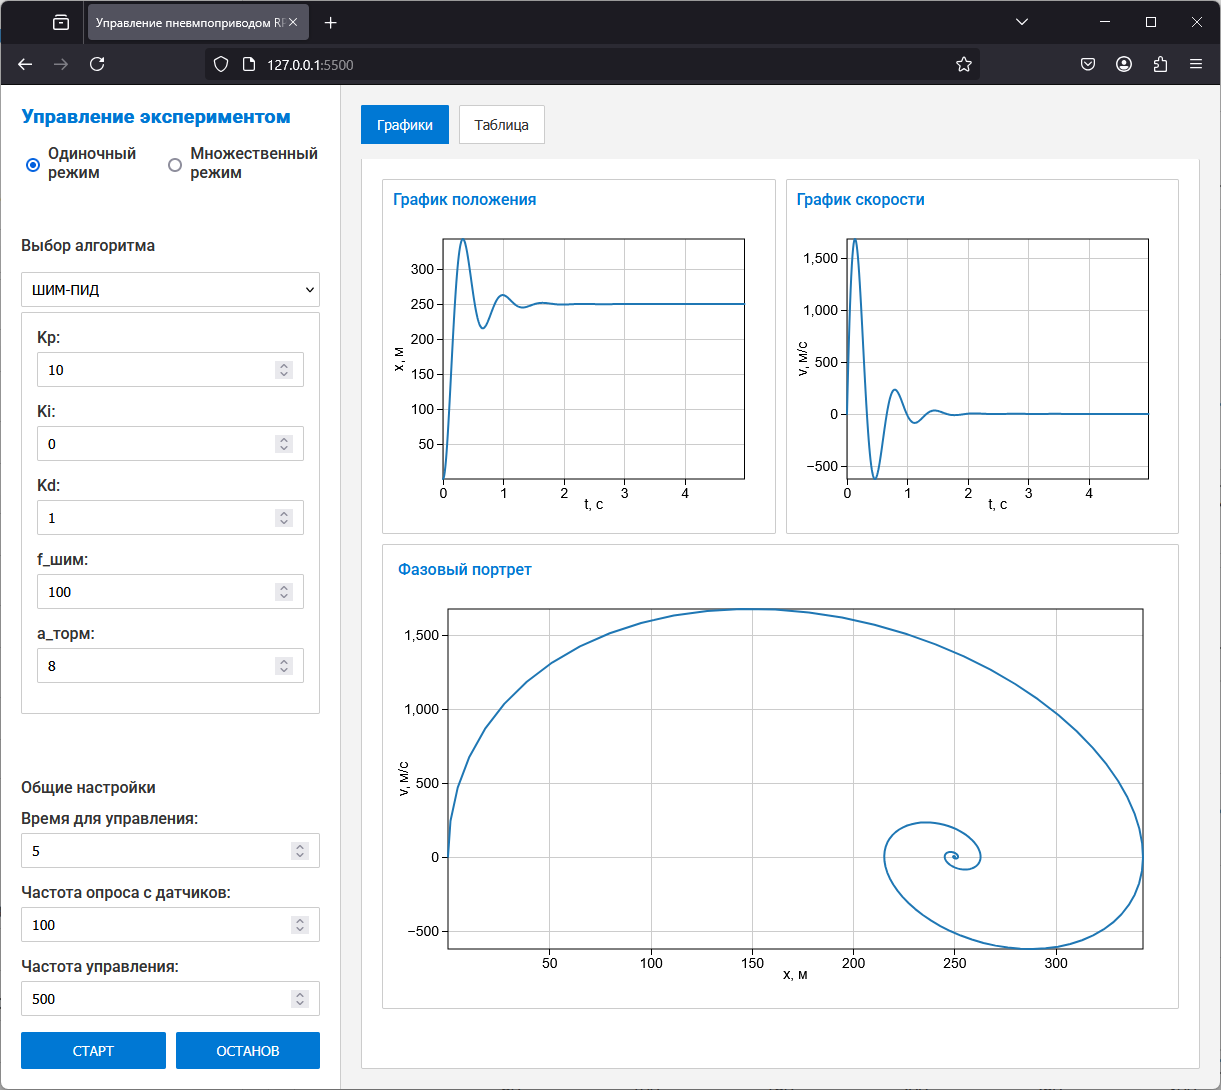
\includegraphics[width=0.85\textwidth]{Снимок экрана 2025-02-27 144410.png}
% 			\scriptsize{Веб-интерфейс системы}

% 			\vspace{0.3em}

% 			\scriptsize
% 			\begin{itemize}
% 				\setlength{\itemsep}{0pt}
% 				\item \textbf{Иерархическая архитектура:}
% 				      \begin{itemize}
% 					      \setlength{\itemsep}{0pt}
% 					      \item \scriptsize Исполнительный уровень (датчики, актуаторы)
% 					      \item \scriptsize Управление в реальном времени (STM32)
% 					      \item \scriptsize Человеко-машинный интерфейс (Raspberry Pi 5)
% 				      \end{itemize}
% 				      %   \item \textbf{Программное обеспечение:}
% 				      %   \begin{itemize}
% 				      % 	\setlength{\itemsep}{0pt}
% 				      % 	\item \scriptsize Алгоритмы управления (C/C++)
% 				      % 	\item \scriptsize Веб-сервер (Flask/Python)
% 				      % 	\item \scriptsize СУБД для хранения экспериментальных данных
% 				      % 	\item \scriptsize REST API для взаимодействия компонентов
% 				      %   \end{itemize}
% 			\end{itemize}
% 		\end{column}
% 	\end{columns}
% \end{frame}

% \begin{frame}{Результаты экспериментов}
% 	\centering
% 	\scriptsize
% 	\begin{tabular}{lccc}
% 		\midrule
% 		\textbf{Метод управления} & $\delta_{\text{rel}}$,~\%     & $\delta_{\text{abs}}$,~\%     & \textbf{Максимальная погрешность}~\% \\
% 		\midrule
% 		ПИД-регулятор с ШИМ       & \cellcolor{green!25}\num{4.3} & \cellcolor{green!25}\num{2.4} & \cellcolor{green!25}\num{10.7}       \\
% 		УСР-И-3                   & \num{6.0}                     & \num{4.0}                     & \num{13.5}                           \\
% 		УСР-И-5                   & \num{5.4}                     & \num{3.3}                     & \num{12.0}                           \\
% 		УСР-И-7                   & \num{7.0}                     & \num{4.6}                     & \num{15.6}                           \\
% 		УСР-Т-3                   & \num{6.7}                     & \num{4.1}                     & \num{14.8}                           \\
% 		УСР-Т-5                   & \num{6.1}                     & \num{3.7}                     & \num{13.8}                           \\
% 		УСР-Т-7                   & \cellcolor{red!25}\num{8.3}   & \cellcolor{red!25}\num{5.3}   & \cellcolor{red!25}\num{18.4}         \\
% 		Нечеткий регулятор        & \num{5.2}                     & \num{3.4}                     & \num{12.5}                           \\
% 		Прогнозное управление     & \num{5.9}                     & \num{3.9}                     & \num{14.5}                           \\
% 		\midrule
% 	\end{tabular}
% 	\vspace{0.1em}

% 	\begin{tabular}{p{3cm}cccccc}
% 		\midrule
% 		\textbf{Метод управления} & $AC^{\text{прог}}$ & $AC^{\text{факт}}$ & $SI^{\text{прог}}$ & $SI^{\text{факт}}$ & $ITAE^{\text{прог}}$,             & $ITAE^{\text{факт}}$,             \\
% 		                          & мм                 & мм                 &                    &                    & ~\si{\milli\meter\squared\second} & ~\si{\milli\meter\squared\second} \\
% 		\midrule
% 		ПИД-регулятор с ШИМ       & \num{0.45}         & \num{0.47}         & \num{32}           & \num{34}           & \num{0.0210}                      & \num{0.0232}                      \\
% 		УСР-И-3                   & \num{1.05}         & \num{1.12}         & \num{12}           & \num{13}           & \num{0.0450}                      & \num{0.0513}                      \\
% 		УСР-И-5                   & \num{0.20}         & \num{0.21}         & \num{8}            & \num{9}            & \num{0.0340}                      & \num{0.0381}                      \\
% 		УСР-И-7                   & \num{0.05}         & \num{0.05}         & \num{18}           & \num{21}           & \num{0.0180}                      & \num{0.0208}                      \\
% 		УСР-Т-3                   & \num{0.12}         & \num{0.13}         & \num{25}           & \num{28}           & \num{0.0260}                      & \num{0.0298}                      \\
% 		УСР-Т-5                   & \num{0.17}         & \num{0.18}         & \num{14}           & \num{16}           & \num{0.0195}                      & \num{0.0222}                      \\
% 		УСР-Т-7                   & \num{0.06}         & \num{0.07}         & \num{12}           & \num{13}           & \num{0.0235}                      & \num{0.0278}                      \\
% 		Нечеткий регулятор        & \num{0.42}         & \num{0.44}         & \num{27}           & \num{31}           & \num{0.0065}                      & \num{0.0073}                      \\
% 		Прогнозное управление     & \num{0.05}         & \num{0.06}         & \num{17}           & \num{19}           & \num{0.0120}                      & \num{0.0138}                      \\
% 		\midrule
% 	\end{tabular}
% \end{frame}

\begin{frame}{Верификация математической модели}
	\begin{columns}
		\begin{column}{0.4\textwidth}
			\begin{block}{\scriptsize \textbf{Параметры верификации}}
				\scriptsize Показатели:
				\begin{itemize}
					\item \scriptsize $R^2$
					\item \scriptsize $RMSE$
				\end{itemize}
				Для всех управляющих структур
			\end{block}

			\vspace{2em}

			\scriptsize
			% \begin{tabular}{lcc}
			% 	\midrule
			% 	\textbf{Управляющая} & $RMSE$,           & $R^2$,       \\
			% 	\textbf{структура}   & \si{\milli\metre} & --           \\
			% 	\midrule
			% 	ПИД с ШИМ            & \num{0.107}       & \num{0.9968} \\
			% 	\hline
			% 	Скользящие           & \num{0.073}       & \num{0.9985} \\
			% 	режимы               &                   &              \\
			% 	\hline
			% 	0				Нечеткое        & \num{0.057}       & \num{0.9972} \\
			% 	управление           &                   &              \\
			% 	\hline
			% 	Прогнозное           & \num{0.035}       & \num{0.9989} \\
			% 	управление           &                   &              \\
			% 	\midrule
			% \end{tabular}
			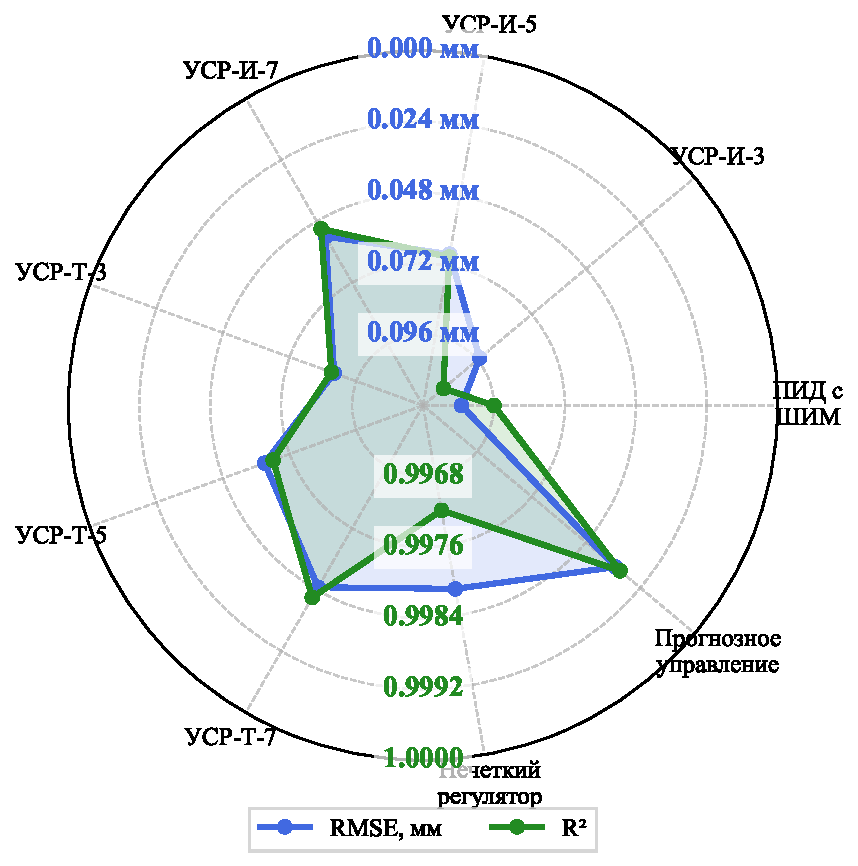
\includegraphics[width=\textwidth]{combined_radar_chart.pdf}

		\end{column}
		\begin{column}{0.6\textwidth}
			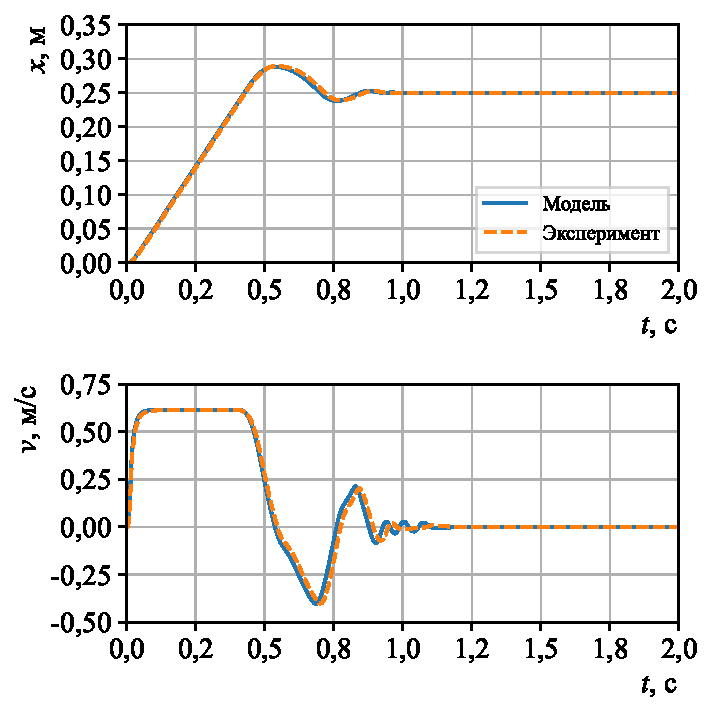
\includegraphics[width=\textwidth]{real_system_transient.pdf}

		\end{column}

	\end{columns}

\end{frame}


% \begin{exampleblock}{Ключевые особенности}
% 	\scriptsize
% 	\begin{itemize}\setlength{\itemsep}{0pt}
% 		\item Прогнозирование будущего поведения системы на основе модели
% 		\item Оптимизация последовательности переключений распределителей
% 		\item Явный учет ограничений на состояния системы
% 		\item Компромисс между точностью и числом переключений
% 		\item Адаптация к изменениям внешних условий
% 	\end{itemize}
% \end{exampleblock}


% \begin{frame}{Методика многокритериальной оптимизации}
% 	\begin{block}{Критерии оптимизации}
% 		\scriptsize
% 		\begin{align*}
% 			AC   & = \eval{\abs{e(t)}}_{t=\infty}                                     \\
% 			ITAE & = \int_{0}^{T} t\abs{e(t)} dt                                      \\
% 			SI   & = \int_0^T \sqrt{\sum_{i=1}^4 \left( \frac{dN_i(t)}{dt} \right)}dt
% 		\end{align*}
% 		% \vspace{-0.3cm}
% 		\begin{itemize}
% 			\footnotesize
% 			\item \scriptsize $AC$ -- точность позиционирования
% 			\item \scriptsize $ITAE$ -- интегральный критерий качества
% 			\item \scriptsize $SI$ -- интенсивность переключений
% 		\end{itemize}
% 	\end{block}
% 	% \begin{columns}
% 	% 	\begin{column}{0.48\textwidth}
% 	% 	\end{column}

% 	% 	\begin{column}{0.48\textwidth}
% 	% 	\end{column}
% 	% \end{columns}
% \end{frame}

\section {Структурно-параметрический синтез позиционного пневмопривода}

\begin{frame}{Двухэтапная методика структурно-параметрического синтеза}
	\centering
	\vspace{-0.5cm}
	\begin{columns}[T]
		\begin{column}{0.48\textwidth}
			\begin{block}{\scriptsize \textbf{Этап 1: Построение фронтов Парето}}
				\scriptsize
				\begin{itemize}
					\item Задание векторов варьируемых параметров
					\item Построение суррогатных (замещающих, аппроксимирующих) моделей
					\item Многокритериальная оптимизация
					\item Построение Парето-фронтов для каждой структуры
				\end{itemize}
			\end{block}
		\end{column}

		\begin{column}{0.48\textwidth}
			\begin{block}{\scriptsize \textbf{Этап 2: Определение параметров}}
				\scriptsize
				\begin{itemize}
					\item Формирование требований к системе
					\item Поиск соответствующих точек на фронтах
					\item Выбор оптимальной структуры
					\item Определение конкретных значений параметров
				\end{itemize}
			\end{block}
		\end{column}
	\end{columns}
	\centering
	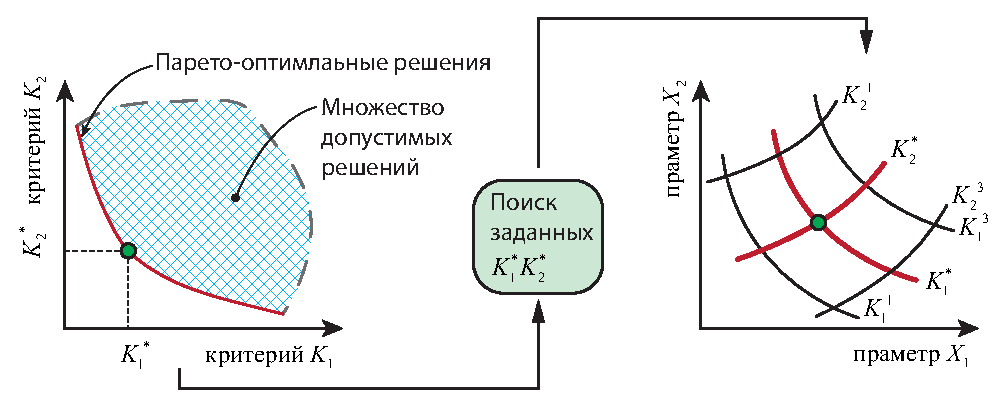
\includegraphics[width=0.8\textwidth]{иллюстрация оптимизации.eps}
\end{frame}

\begin{frame}{Этап 1: Построение фронтов Парето}
	% \setlength{\columnsep}{5pt}
	\begin{columns}[]
		\begin{column}{0.5\textwidth}
			\vspace{-0.3cm}
			\begin{block}{\scriptsize \textbf{Критерии оптимизации}}
				\scriptsize
				$$ AC = \eval{\abs{e(t)}}_{t=\infty}$$
				где $e(t)$ -- ошибка позиционирования \\
				$$ITAE = \int_{0}^{T} t\abs{e(t)} dt$$\\
				где $T$ -- время эксперимента \\
				$$ SI = \int_0^T \sqrt{\sum_{i=1}^4 \left( \frac{dN_i(t)}{dt} \right)}dt$$
				где $N_i(t)$ -- переключение i-го распределителя
				\begin{itemize}
					\footnotesize
					\item \scriptsize $AC$ -- точность позиционирования
					\item \scriptsize $ITAE$ -- интегральный критерий качества
					\item \scriptsize $SI$ -- интенсивность переключений
				\end{itemize}
			\end{block}

		\end{column}

		\begin{column}{0.5\textwidth}
			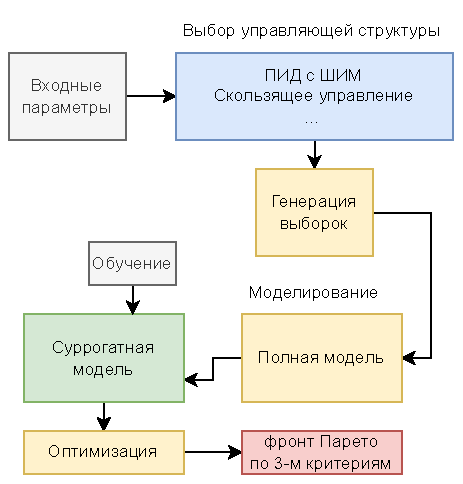
\includegraphics[width=0.9\textwidth]{блоксхема-прямой-задачи.pdf}
		\end{column}
	\end{columns}
\end{frame}


\begin{frame}{Этап 2: Определение параметров (обратная задача)}
	\begin{columns}
		\begin{column}{0.48\textwidth}
			\vspace{-0.2cm}
			\begin{block}{Постановка задачи}
				\scriptsize
				\begin{equation*}
					\mathbf{p}^* = \arg\min_{\mathbf{p}} \norm{\mathbf{y}(\theta) - \mathbf{p}^*}
				\end{equation*}
				\scriptsize где $\mathbf{p}^*$ -- искомый вектор параметров управления; $\theta$ -- требуемые значения критериев $AC$, $ITAE$, $SI$
			\end{block}

			% \begin{block}{Алгоритм}
			% 	\begin{enumerate}
			% 		\item \scriptsize Задание требуемых значений критериев $\mathbf{p} = [AC, ITAE, SI]$
			% 		\item \scriptsize Формирование целевой функции как взвешенной суммы относительных отклонений
			% 		\item \scriptsize Поиск оптимального набора параметров $\mathbf{p}^*$ методом градиентного спуска
			% 		\item \scriptsize Верификация полученного решения
			% 	\end{enumerate}
			% \end{block}

		\end{column}

		\begin{column}{0.52\textwidth}
			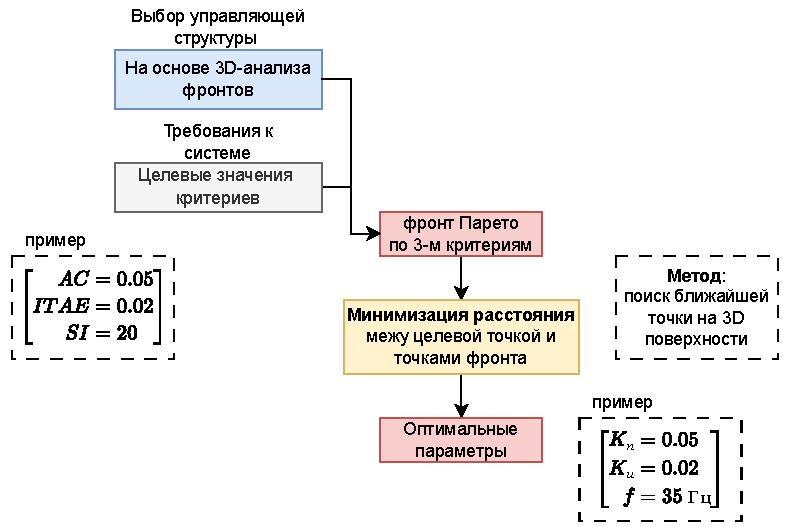
\includegraphics[width=1.1\textwidth]{блоксхема-обратной-задачи.pdf}
		\end{column}
	\end{columns}
\end{frame}

\begin{frame}
	\frametitle{Парето-фронты для различных управляющтх структур}
	% \hspace{-1.75cm}
	% \vspace{0.5cm}
	\hspace*{0pt}\makebox[\linewidth][c]{
		\begin{tabular}{ccc}
			\scriptsize
			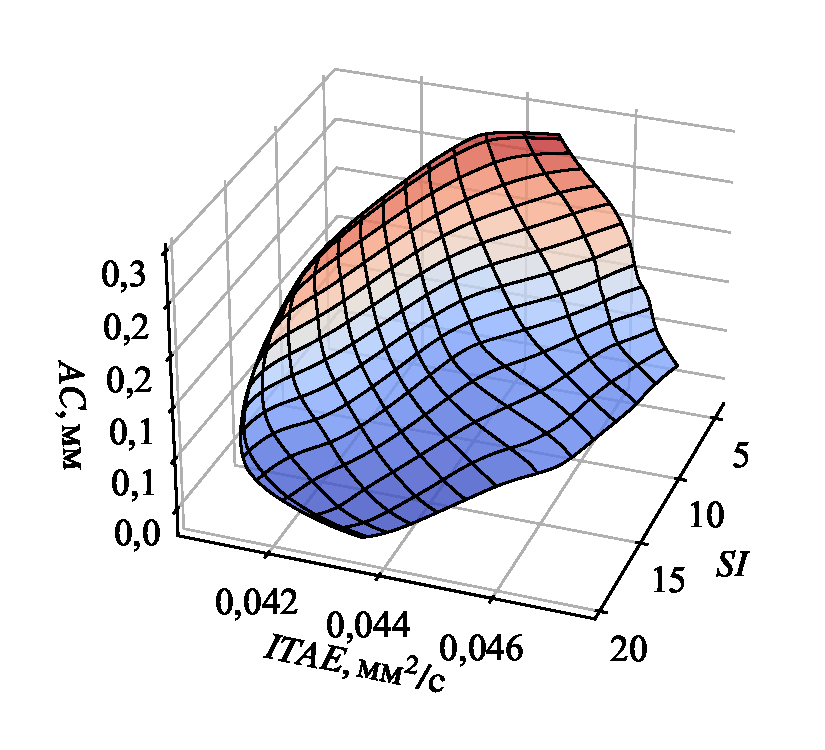
\includegraphics[width=0.3\textwidth]{paretos/Нечеткий.pdf} & 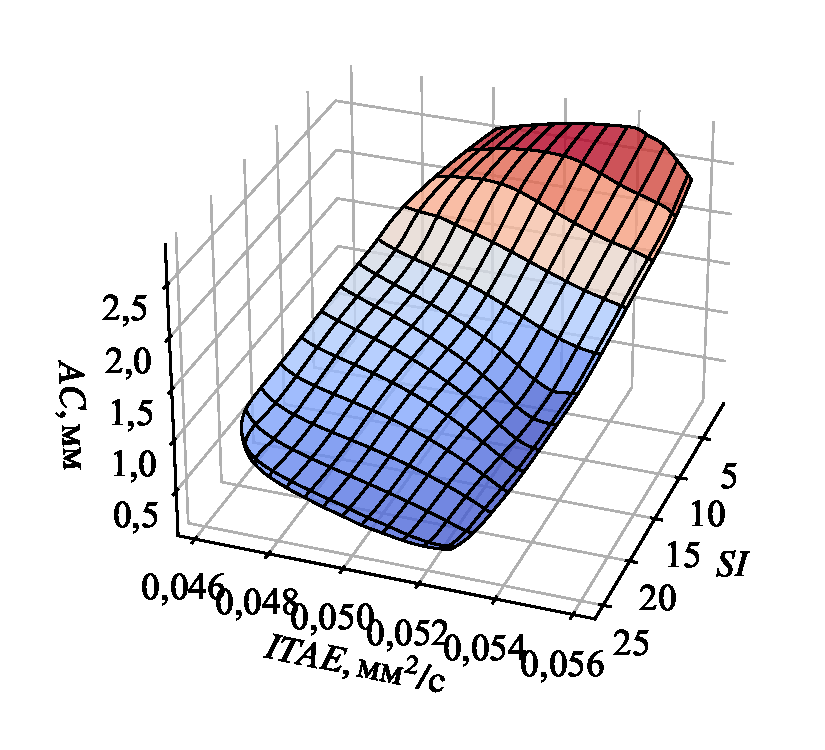
\includegraphics[width=0.3\textwidth]{paretos/УСР-И-3.pdf} & 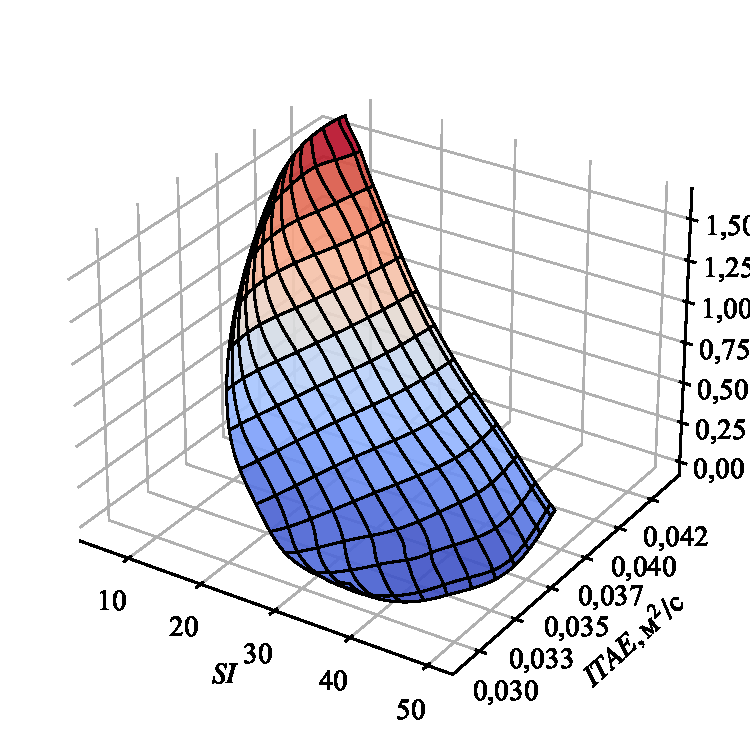
\includegraphics[width=0.3\textwidth]{paretos/ПИД+ШИМ.pdf} \\
			\scriptsize Нечеткая логика                                 & \scriptsize УСР интегральная 3-х режимная                  & \scriptsize Мод. ПИД с ШИМ                                 \\
			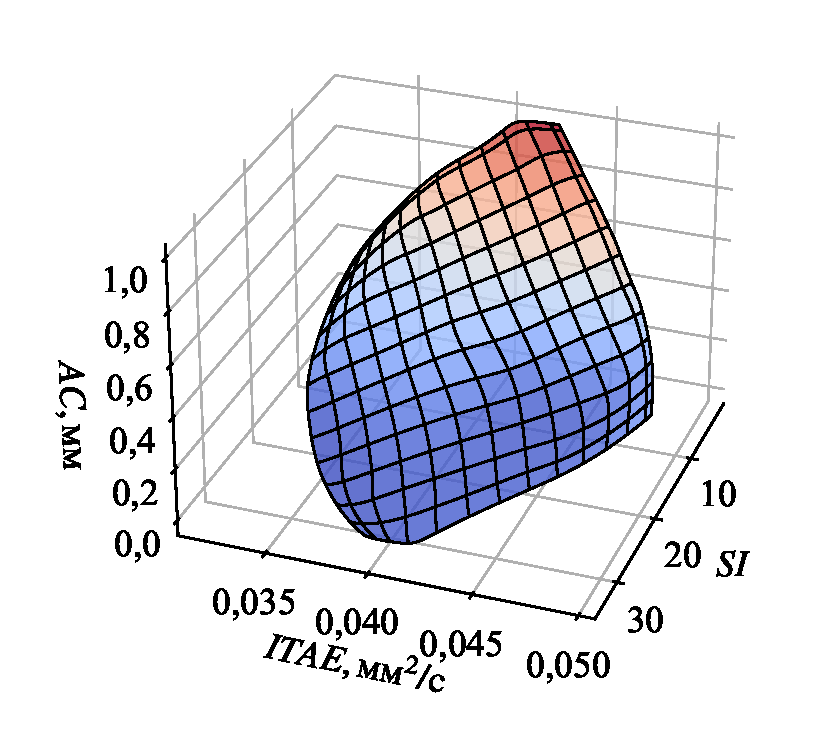
\includegraphics[width=0.3\textwidth]{paretos/УСР-И-5.pdf}  & 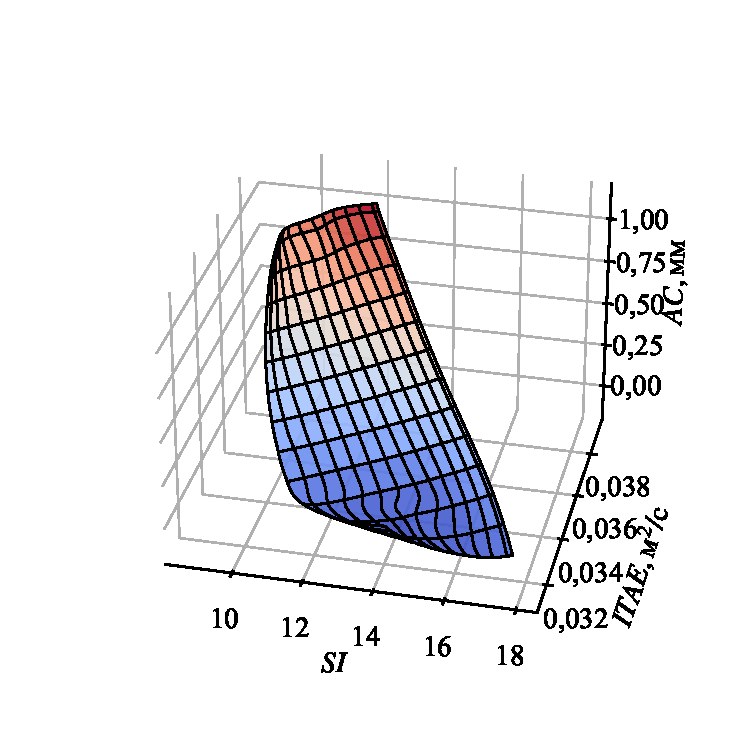
\includegraphics[width=0.3\textwidth]{paretos/MPC.pdf}     & 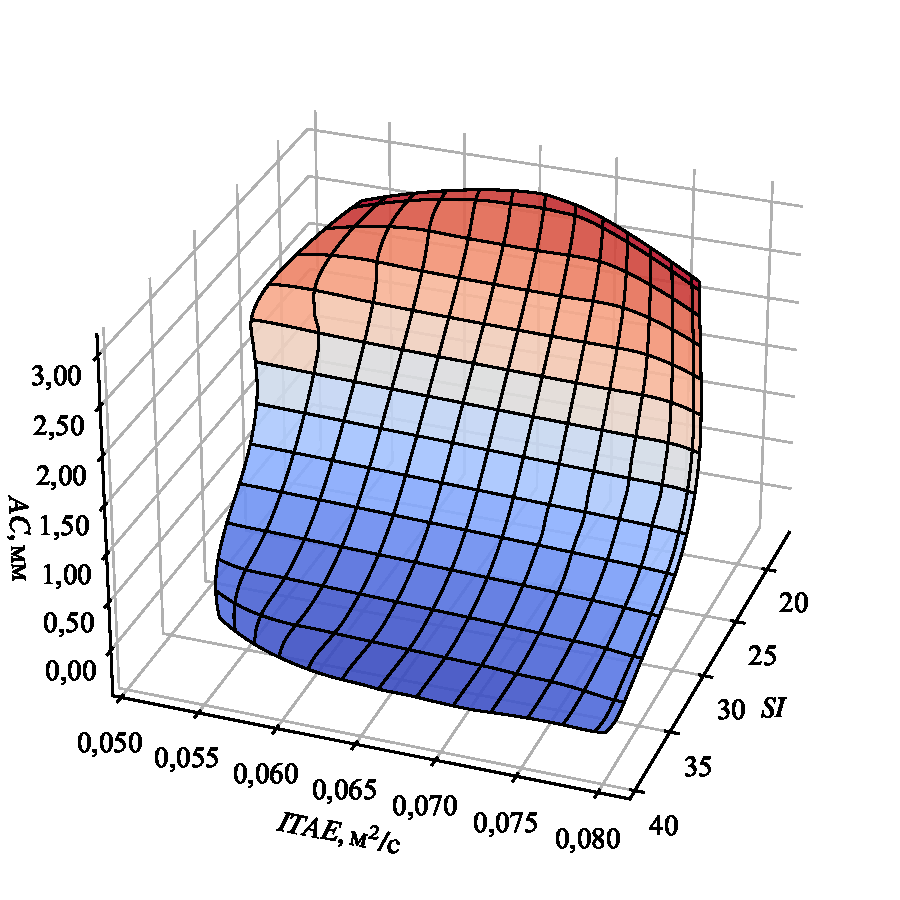
\includegraphics[width=0.3\textwidth]{paretos/УСР-Т-3.pdf} \\
			\scriptsize  УСР интегральная 5-и режимная                  & \scriptsize Прогнозное управление                          & \scriptsize УСР теримнальная 3-х режимная                  \\
			% 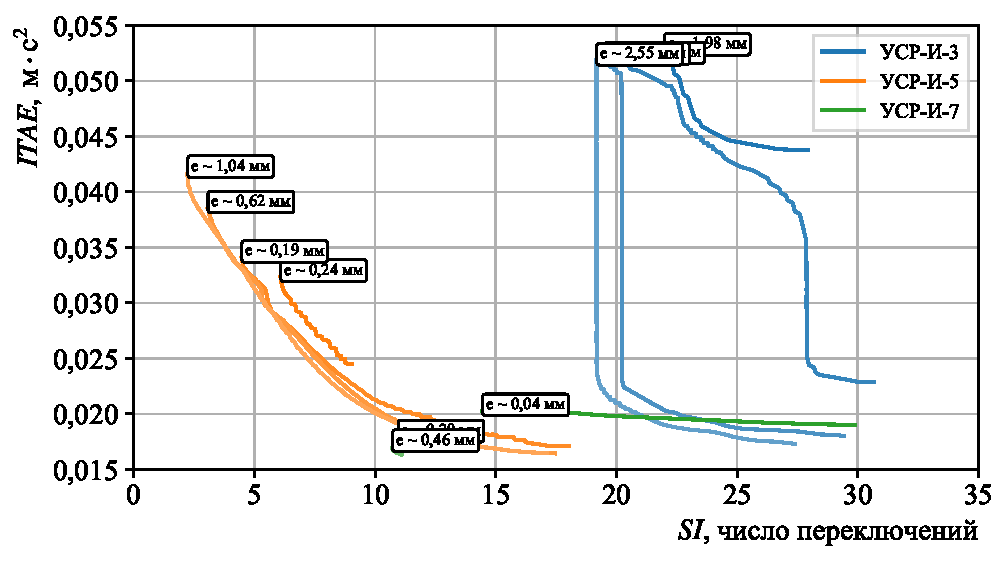
\includegraphics[width=0.5\textwidth]{smc_integral_pareto.pdf} & 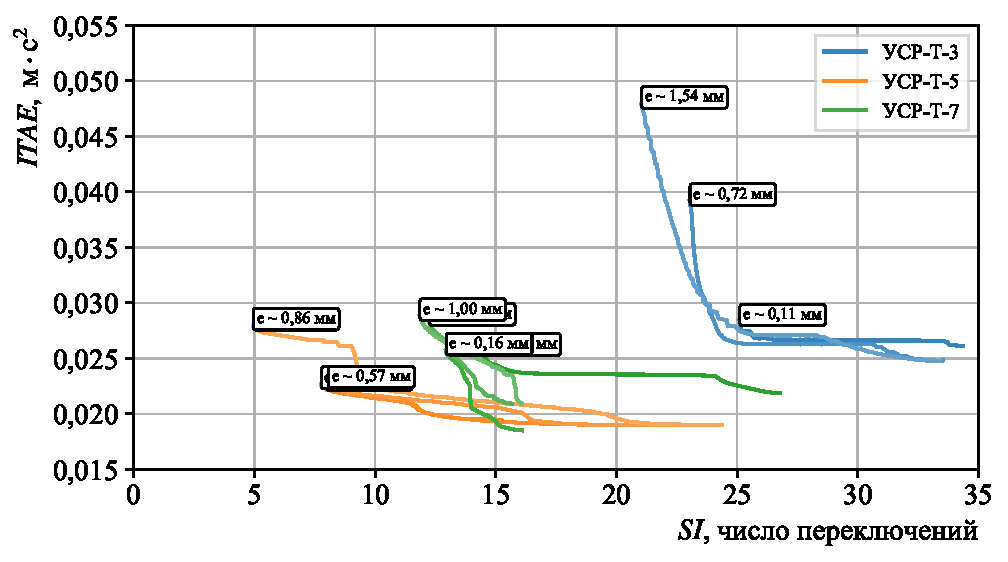
\includegraphics[width=0.5\textwidth]{smc_terminal_pareto.pdf} \\
			% \scriptsize УСР интрегральная                                  & \scriptsize УСР терминальная                                   \\
		\end{tabular}
	}
\end{frame}

\begin{frame}{Получение результатов обратной задачи}
	\begin{columns}
		\begin{column}{0.48\textwidth}
			\begin{block}{\scriptsize Этапы}
				\scriptsize
				\begin{itemize}
					\item Генерация тестовых данных в пространстве критериев
					\item Определении по методике обратной задачи оптимальных параметров
					\item Расчет критериев для полученных параметров по полной модели
					\item Вычисление относительных погрешностей
				\end{itemize}
			\end{block}
		\end{column}

		\begin{column}{0.52\textwidth}
			\begin{block}{\scriptsize Показатели оценки}
				\scriptsize
				\begin{center}
					\begin{equation*}
						\begin{aligned}
							\delta_{\text{rel}} & = \frac{1}{m} \sum_{i=1}^{m} \frac{ \left| J_i^{\text{прог}} - J_i^{\text{факт}} \right|}{J_{\text{факт}}} \cdot 100\%,                 \\
							\delta_{\text{abs}} & = \frac{1}{m} \sum_{i=1}^{m} \frac{ \left| J_i^{\text{прог}} - J_i^{\text{факт}} \right|}{J_{\text{max}} - J_{\text{min}}} \cdot 100\%, \\
						\end{aligned}
					\end{equation*}
				\end{center}
				\begin{itemize}
					\item $J_i^{\text{прог}}$ -- прогнозируемое значение i-го критерия оптимизации
					\item $J_i^{\text{факт}}$ -- фактическое значение i-го критерия оптимизации
					\item $J_i^{\max}$ и $J_i^{\min}$ -- максимальное и минимальное значения i-го критерия в обучающей выборке

				\end{itemize}
			\end{block}
		\end{column}
	\end{columns}
\end{frame}

\begin{frame}{Результаты обратной задачи}
	\centering
	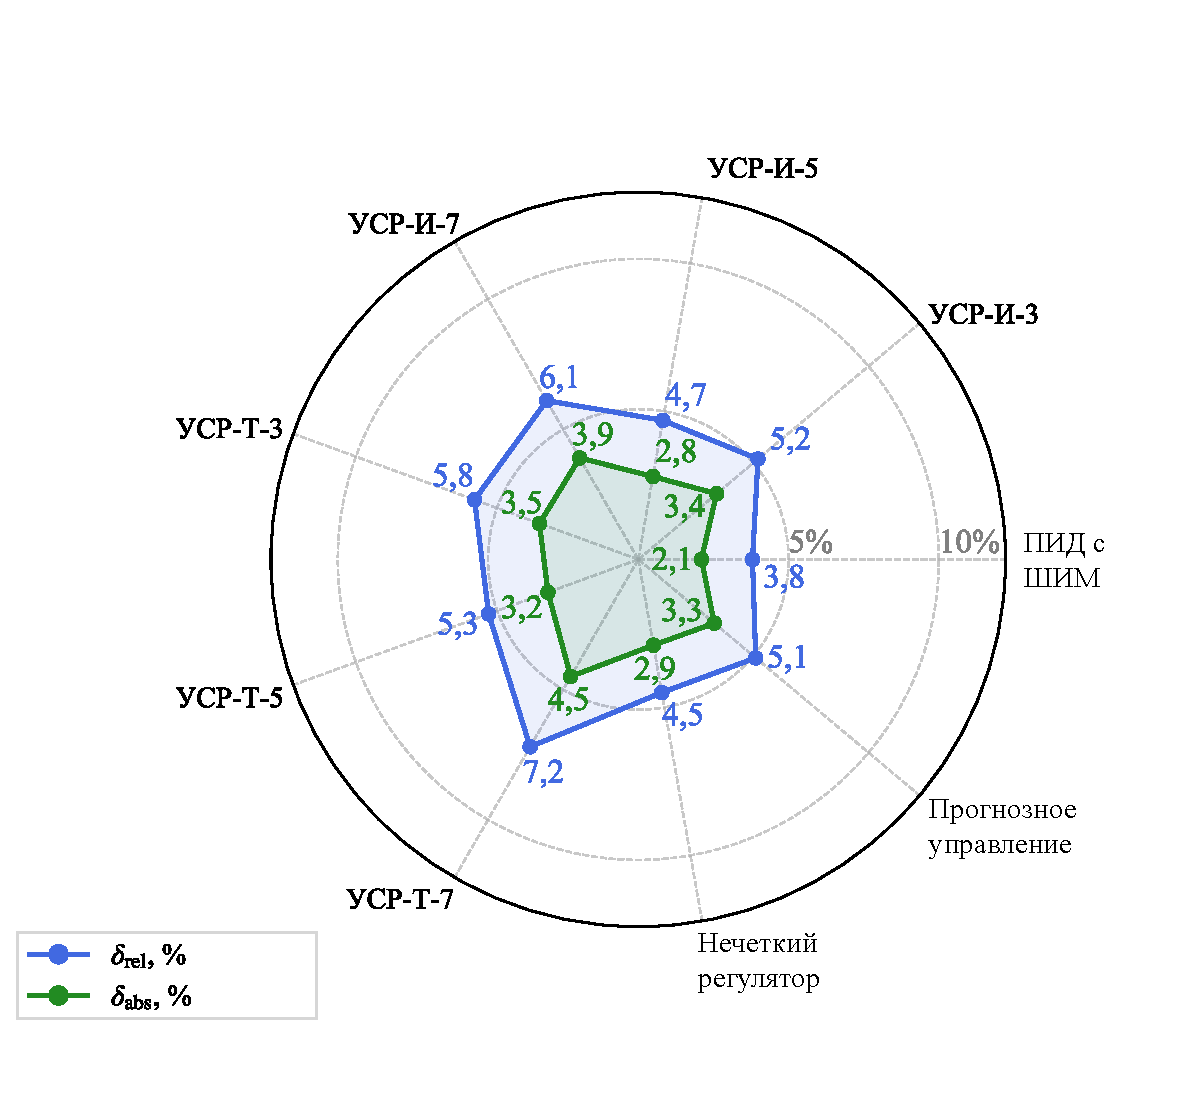
\includegraphics[width=0.8\textwidth]{radar_comparison_chart.eps}
	% \scriptsize
	% \begin{tabular}{lccc}
	% 	\midrule
	% 	\textbf{Метод управления} & $\delta_{\text{rel}}$,~\%     & $\delta_{\text{abs}}$,~\%     & \textbf{Максимальная погрешность}~\% \\
	% 	\midrule
	% 	ПИД-регулятор с ШИМ       & \cellcolor{green!25}\num{3.8} & \cellcolor{green!25}\num{2.1} & \cellcolor{green!25}\num{9.2}        \\
	% 	УСР-И-3                   & \num{5.2}                     & \num{3.4}                     & \num{11.6}                           \\
	% 	УСР-И-5                   & \num{4.7}                     & \num{2.8}                     & \num{10.3}                           \\
	% 	УСР-И-7                   & \num{6.1}                     & \num{3.9}                     & \num{13.5}                           \\
	% 	УСР-Т-3                   & \num{5.8}                     & \num{3.5}                     & \num{12.7}                           \\
	% 	УСР-Т-5                   & \num{5.3}                     & \num{3.2}                     & \num{11.9}                           \\
	% 	УСР-Т-7                   & \cellcolor{red!25}\num{7.2}   & \cellcolor{red!25}\num{4.5}   & \cellcolor{red!25}\num{15.8}         \\
	% 	Нечеткий регулятор        & \num{4.5}                     & \num{2.9}                     & \num{10.8}                           \\
	% 	Прогнозное управление     & \num{5.1}                     & \num{3.3}                     & \num{12.5}                           \\
	% 	\midrule
	% \end{tabular}
\end{frame}



\begin{frame}{Рекомендации по выбору алгоритмов управления}
	\centering
	\vspace{-3em}
	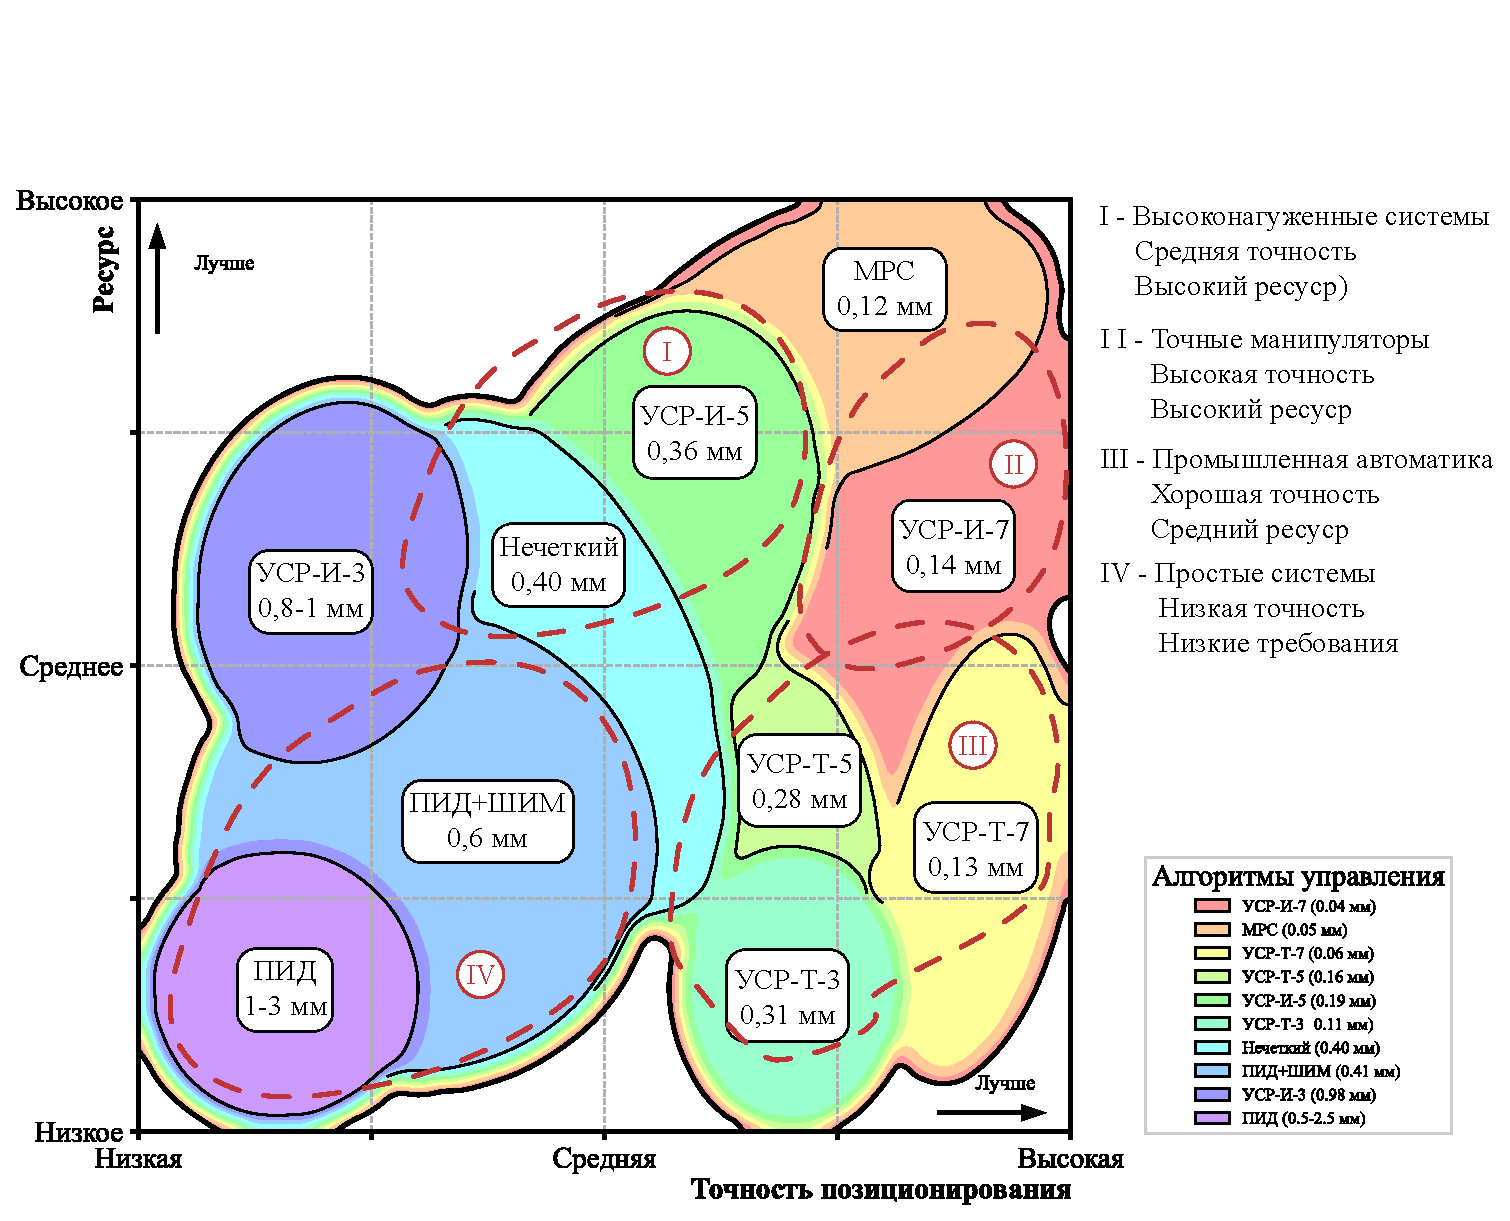
\includegraphics[width=1\textwidth]{algorithm_map.eps}
	% \fontsize{7.5pt}{8pt}\selectfont
	% \begin{columns}
	% 	\begin{column}{0.48\textwidth}
	% 		\begin{tabular}{|p{0.5\linewidth}|p{0.45\linewidth}|}
	% 			\hline
	% 			\textbf{Приоритет}                               & \textbf{Рекомендуемые алгоритмы} \\
	% 			\hline
	% 			\textbf{Высокая точность} \newline (до 0.1 мм)   &
	% 			УСР-И-7 (0.04 мм) \newline
	% 			МРС (0.05 мм) \newline
	% 			УСР-Т-7 (0.06 мм)                                                                   \\
	% 			\hline
	% 			\textbf{Средняя точность} \newline (0.1--0.5 мм) &
	% 			УСР-Т-3 (0.11 мм) \newline
	% 			УСР-Т-5 (0.16 мм) \newline
	% 			УСР-И-5 (0.19 мм) \newline
	% 			Нечеткий (0.40 мм) \newline
	% 			ПИД+ШИМ (0.41 мм)                                                                   \\
	% 			\hline
	% 			\textbf{Низкая точность} \newline (>0.5 мм)      &
	% 			УСР-И-3 (0.98 мм) \newline
	% 			ПИД (0.5--2.5 мм)                                                                   \\
	% 			\hline
	% 		\end{tabular}
	% 	\end{column}
	% 	\begin{column}{0.52\textwidth}
	% 		\begin{tabular}{|p{0.5\linewidth}|p{0.45\linewidth}|}
	% 			\hline
	% 			\textbf{Минимум переключений}                     &
	% 			УСР-И-5 (5 перекл.) \newline
	% 			МРС (5 перекл., 0.47 мм)                            \\
	% 			\hline
	% 			\textbf{Оптимальная динамика} \newline (min ITAE) &
	% 			Нечеткий (0.006 мм²с) \newline
	% 			МРС (0.012 мм²с) \newline
	% 			УСР-И-7 (0.019 мм²с)                                \\
	% 			\hline
	% 		\end{tabular}

	% 		\vspace{0.2em}

	% 		\textbf{Выбор для типовых применений:}

	% 		\begin{tabular}{p{0.5\linewidth}p{0.45\linewidth}}
	% 			\textit{Точные манипуляторы:}       & УСР-И-7, МРС      \\
	% 			\textit{Промышленная автоматика:}   & УСР-Т-5, Нечеткий \\
	% 			\textit{Высоконагруженные системы:} & УСР-И-5, МРС      \\
	% 			\textit{Простые системы:}           & ПИД+ШИМ, УСР-И-3  \\
	% 		\end{tabular}
	% 	\end{column}
	% \end{columns}
\end{frame}

